\documentclass[11pt]{extarticle} 
\usepackage{unicode-math}
\usepackage{mathrsfs}
\usepackage{amsthm,graphicx,xcolor,natbib,enumitem,booktabs,tabularx}
\usepackage[paperwidth=126mm, paperheight=96mm, top=5mm, bottom=5mm, right=5mm, left=5mm]{geometry}
\pagenumbering{gobble}

\usepackage[BoldFont,SlantFont]{xeCJK}  
\xeCJKsetemboldenfactor{2}
\setCJKmainfont{cwTeX Q Yuan Medium}

\usepackage{hyperref}
\hypersetup{
    colorlinks,
    linkcolor={red!50!black},
    citecolor={blue!60!black},
    urlcolor={blue!60!black}
}

\newcommand{\ds}{\displaystyle}
\newcommand{\ie}{\;\Longrightarrow\;}
\newcommand{\ifff}{\;\Longleftrightarrow\;}
\newcommand{\mi}{\mathrm{i}}
\DeclareMathOperator*{\dom}{dom}
\DeclareMathOperator*{\codom}{codom}
\DeclareMathOperator*{\ran}{ran}
\newcommand{\floor}[1]{\lfloor #1 \rfloor}
\newcommand{\ceil}[1]{\lceil #1 \rceil}
\newcommand{\Set}[2]{\big\{ \ #1\ \big|\ #2\ \big\}}
\newcommand{\pdiff}[2]{\frac{\partial\hfil#1\hfil}{\partial #2}}
\newcommand{\vx}{\symbfup{x}}
\newcommand{\vd}{\symbfup{d}}
\newcommand{\vg}{\symbfup{g}}
\newcommand{\vH}{\symbfup{H}}
\newcommand{\va}{\symbfup{a}}
\newcommand{\vb}{\symbfup{b}}
\newcommand{\vbb}{\symbfup{\beta}}
\newcommand{\vS}{\symbfup{S}}
\newcommand{\vR}{\symbfup{R}}
\newcommand{\vV}{\symbfup{V}}
\newcommand{\ve}{\symbfup{e}}
\newcommand{\vr}{\symbfup{r}}
\newcommand{\vZero}{\symbfup{0}}

\DeclareMathOperator\prb{{\sf P}}
\DeclareMathOperator\expc{{\sf E}}
\DeclareMathOperator\var{var}
\DeclareMathOperator\cov{cov}
\DeclareMathOperator\cor{cor}
\DeclareMathOperator*{\argmax}{\arg\!\max}
\DeclareMathOperator*{\argmin}{\arg\!\min}
\DeclareMathOperator*{\im}{Im}
\DeclareMathOperator*{\re}{Re}
\DeclareMathOperator*{\conv}{conv}
\DeclareMathOperator*{\proj}{proj}
\DeclareMathOperator*{\tr}{tr}
\DeclareMathOperator*{\diag}{diag}
\DeclareMathOperator*{\epi}{epi}
\DeclareMathOperator*{\dist}{dist}
\DeclareMathOperator*{\inte}{int}
\DeclareMathOperator*{\relint}{relint}

\theoremstyle{definition}
\newtheorem*{dfn}{Definition}
\newtheorem*{prp}{Property}
\newtheorem*{thm}{Theorem}
\newtheorem*{ex}{Example}
\newtheorem*{sol}{Solution}
\newtheorem*{prf}{Proof}

\newcommand\scalemath[2]{\scalebox{#1}{\mbox{\ensuremath{\displaystyle #2}}}}

\begin{document}
\title{\texorpdfstring{\vspace{15mm} Operations Research\\ 08. Portfolio Optimization}{Operations Research\\ 08. Portfolio Optimization}} 
\author{}
\date{}
\maketitle
\newpage

\section*{Classical PO: Mean-Variance (MV) Criterion}

\begin{itemize}\setlength\itemsep{0em}
  \item Assets evolve from time $0$ to time $1$ for one period
  \item $s$: \# of risky assets 
  \item $\vS_0\equiv(S_{1, 0}, S_{2, 0}, \ldots, S_{s, 0})^\top\not=\vZero$: the constant price vector at time $0$
  \item $\vS_1\equiv(S_{1, 1}, S_{2, 1}, \ldots, S_{s, 1})^\top$: the random price vector at time $1$
  \item $\vx\equiv(x_1, x_2, \ldots, x_s)^\top$: the proportion vector of the time-$0$ wealth invested in each asset; $\ds\sum_{i=1}^s x_i = 1$.
  \item $\vR\equiv(R_1, R_2, \ldots, R_s)^\top$: the random vector representing the rate of return on the assets; $\ds R_i = \frac{S_{i, 1}}{S_{i, 0}}$
  \item $w$: the (constant) wealth at time $0$
  \item $W$: the (random) wealth at time $1$; $\ds W = \bigg(\sum_{i=1}^s x_i R_i\bigg) w = \vx^\top\vR\,w$ (For asset $S_i$, $\ds\frac{x_i w}{S_{i, 0}}$ denotes the ``quantity'' allocated at time $0$; so at time $1$ this part of wealth becomes $\ds\frac{x_i w}{S_{i, 0}}\,S_{i, 1} = x_i R_i w$)  
  \item $\vr\equiv\expc{\vR} = (r_1, r_2, \ldots, r_s)^\top$: the (constant) mean vector of $\vR$; $\ds r_i = \expc{R_i}$
  \item $\vV\equiv\cov{\vR}\equiv\expc\{(\vR - \vr)(\vR - \vr)^\top\}$: the (constant) covariance matrix of $\vR$; $\vV$ is symmetric positive semidefinite $s\times s$ matrix
  \item $\expc W = \expc\{\vx^\top\vR\} = \vx^\top\vr = \mu$
  \item $\sigma^2 = \var W = \var\{\vx^\top\vR\} = \expc\{\vx^\top(\vR - \vr)(\vR - \vr)^\top\vx\} = \vx^\top\vV\vx$
\end{itemize}

\subsection*{(Classical) Mean-Variance Portfolio Optimization}
\noindent ``For some fixed mean rate of return $\mu = \expc\{\vx^\top\vR\}$, try to minimize the variance $\sigma^2 = \var\{\vx^\top\vR\}$ of the return over portfolios $\vx$''

\section*{MV: All Risky Assets}

\begin{align*}
  \min_{\vx}\,\frac{1}{2}\,\vx^\top\vV\vx\quad\text{s.t.}\quad\begin{cases}\vx^\top\ve = 1 \\\vx^\top\vr = \mu\end{cases}\quad \ve\equiv\underbrace{(1, 1, \ldots, 1)^\top}_{\text{$s$ items}}
\end{align*}

\begin{itemize}\setlength\itemsep{0em}
  \item $\vV$ is symmetric, positive definite, so $\vV^{-1}$ also is
  \item Set $\ds\mathcal{L}\equiv\frac{1}{2}\,\vx^\top\vV\vx + \lambda\,(1 - \vx^\top\ve) + \nu\,(\mu - \vx^\top\vr)$ with Lagrange multipliers $\lambda$, $\nu$
  \item By $\ds\frac{\partial\mathcal{L}}{\partial\vx} = \vV\vx - \lambda\,\ve - \nu\,\vr = 0\ie\vx = \lambda\,\vV^{-1}\ve + \nu\,\vV^{-1}\vr\\ \ie\vx^\top = \lambda\,\ve^\top\left(V^{-1}\right)^\top + \nu\,\vr^\top\left(V^{-1}\right)^\top = \lambda\,\ve^\top\vV^{-1} + \nu\,\vr^\top\vV^{-1}$ 
  \item Substitute into $\ds\begin{cases}\vx^\top\ve = 1 \\\vx^\top\vr = \mu\end{cases}\ie\begin{cases}\lambda\,\ve^\top\vV^{-1}\ve + \nu\,\vr^\top\vV^{-1}\ve = 1 \\ \lambda\,\ve^\top\vV^{-1}\vr + \nu\,\vr^\top\vV^{-1}\vr = \mu\end{cases}$
\end{itemize}

\newpage

\begin{itemize}\setlength\itemsep{0em}
  \item Set $\alpha = \ve^\top\vV^{-1}\ve,\;$ $\beta = \vr^\top\vV^{-1}\ve = \ve^\top\vV^{-1}\vr,\;$ $\gamma = \vr^\top\vV^{-1}\vr,\;$ $\delta\equiv\alpha\gamma - \beta^2\;$, then 
    \begin{align*}
      \begin{cases}\lambda\,\ve^\top\vV^{-1}\ve + \nu\,\vr^\top\vV^{-1}\ve = 1 \\ \lambda\,\ve^\top\vV^{-1}\vr + \nu\,\vr^\top\vV^{-1}\vr = \mu\end{cases}
    \end{align*}
    becomes 
    \begin{align*}\begin{cases}\lambda\alpha + \nu\beta = 1 \\ \lambda\beta + \nu\gamma = \mu\end{cases}
    \end{align*}
    Solutions: $\ds\lambda = \frac{\gamma - \beta\mu}{\delta},\;$ $\ds\gamma = \frac{\alpha\mu - \beta}{\delta}$
  \item If $\vr\not=c\,\ve$, $c\in\mathbb{R}$, then from the positive-definiteness of $\vV^{-1}$ 
    \begin{align*}
      &(\vr - c\,\ve)^\top\vV^{-1}(\vr - c\,\ve) > 0 \\
      &\ie\vr^\top\vV^{-1}\vr - c\,\vr^\top\vV^{-1}\ve - c\,\ve\vV^{-1}\vr + c^2\,\ve^\top\vV^{-1}\ve^\top > 0 \\
      &\ie \gamma-2\,c\,\beta + c^2\,\alpha > 0 \\
      &\ie-\delta = \beta^2 - \gamma\alpha < 0
    \end{align*}
\end{itemize}

\newpage

\begin{itemize}\setlength\itemsep{-2mm}
  \item The relation of $\sigma$ with $\mu$: 
    \begin{align*}
      \sigma^2 &= \vx^\top\vV\vx = \vx^\top\vV(\lambda\vV^{-1}\ve + \nu\vV^{-1}\vr) = \lambda(\vx^\top\ve) + \nu(\vx^\top\vr) \\
      &= \lambda + \nu\mu = \frac{\gamma - \beta\mu}{\delta} + \nu\frac{\alpha\mu-\beta}{\delta} = \frac{\alpha\mu^2 - 2\beta\mu + \gamma}{\delta}\\
      &\ie\frac{\sigma^2}{\left(\frac{1}{\sqrt{\alpha}}\right)^2} - \frac{\left(\mu - \frac{\beta}{\alpha}\right)^2}{\left(\frac{\sqrt{\delta}}{\alpha}\right)^2} = 1
    \end{align*}
  \item Hyperbola $(x, y)$ 
    \begin{align*}
      \text{equation:}\quad &\frac{(x - h)^2}{a^2} - \frac{(y - k)^2}{b^2} = 1 \\
      \text{asymptotes:}\quad &(y - k) =\pm\frac{b}{a}(x - h)
    \end{align*}
  \item Here we have $(\sigma, \mu)$ with $\ds a = \frac{1}{\sqrt{\alpha}}$, $\ds b = \frac{\sqrt{\delta}}{\alpha}$, $\ds h = 0$, $\ds k = \frac{\beta}{\alpha}$, the asymptotes are $\ds\left(\mu - \frac{\beta}{\alpha}\right) = \pm\frac{\frac{\sqrt{\delta}}{\alpha}}{\frac{1}{\sqrt{\alpha}}}\sigma$ $\ie$ $\ds \mu = \frac{\beta}{\alpha} \pm\sqrt{\frac{\delta}{\alpha}}\sigma$
\end{itemize}

\begin{itemize}\setlength\itemsep{-1em}
  \item Global minimum-variance portfolio $\vx_g$
    \vspace{-1em}
    \begin{itemize}\setlength\itemsep{0em}
      \item First find $\mu_g$ that minimizes $\ds\sigma^2 = \frac{\alpha\mu^2 - 2\beta\mu + \gamma}{\delta}$: \\ By differentiation $\ds 2\alpha\mu_g - 2\beta = 0\ie\mu_g = \frac{\beta}{\alpha}$
      \item $\ds\lambda_g = \frac{\gamma - \beta\mu_g}{\delta} = \frac{\gamma-\beta\frac{\beta}{\alpha}}{\delta} = \frac{\gamma\alpha - \beta^2}{\alpha\delta} = \frac{1}{\alpha}$ \\ $\ds\nu_g = \frac{\alpha\mu_g - \beta}{\delta} = \frac{\beta - \beta}{\delta} = 0$ \\ so $\ds\vx_g = \lambda_g\,\vV^{-1}\ve + \nu_g\,\vr^\top\vV^{-1} = \frac{1}{\alpha}\vV^{-1}\ve$
    \end{itemize}
  \item Diversified portfolio: $\ds\vx_d\equiv\frac{1}{\beta}\vV^{-1}\vr$, then the expected return $\ds\mu_d = \vx^\top_d\vr = \frac{1}{\beta}\vr^\top\vV^{-1}\vr = \frac{\gamma}{\beta}$
\end{itemize}

\noindent$\ds\vx = \lambda\vV^{-1}\ve + \nu\vV^{-1}\vr = \lambda\,\alpha\,\vx_g + \nu\,\beta\,\vx_d$, so {\bf every portfolio is the convex combination of $\vx_g$ and $\vx_d$}: note that $\ds\lambda\alpha + \nu\beta = 1$ (constraint $\ds\vx^\top\ve = 1$) ! 

\newpage

\begin{figure}[!htbp]
  \centering
  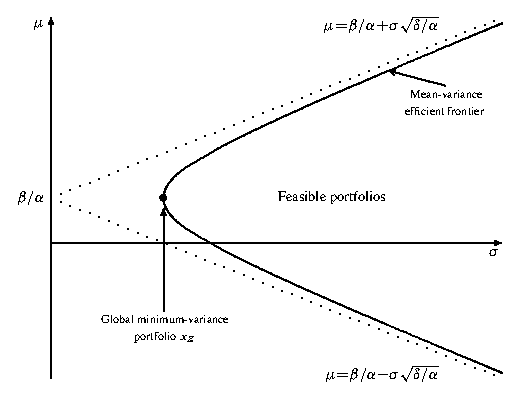
\includegraphics[scale=1.1,page=1]{fig/sfm.pdf}
  \caption{The Case of All Risky Assets}
  \label{fig:mv1}
\end{figure}

\newpage

\begin{thm}[Mutual Fund Theorem]
  Any minimum-variance portfolio is equivalent to investing in the convex combination of $\vx_g$ and $\vx_d$.
\end{thm}

\begin{thm}
  Diversified portfolio $\vx_d$ is the portfolio that maximize $\ds s(\vx)\equiv\frac{\vx^\top\vr}{\sqrt{\vx^\top\vV\vx}}$.
\end{thm}

\begin{prf}
  \begin{itemize}
    \item[]
    \item $\ds\max\,s(\vx)\equiv\max\,\log(s(\vx))$ s.t. $\ds\vx^\top\ve = 1$ 
    \item Change of variable: $\ds\vx^\top\vr = \mu \ie \\ \log(s(\vx)) = \log\frac{\mu}{\sqrt{\frac{\alpha\mu^2 - 2\beta\mu + \gamma}{\delta}}} \equiv f(\mu)$ with $\mu > 0$
    \item $\ds f'(\mu) = \frac{\gamma - \beta\mu}{\mu\left(\alpha\left(\mu - \frac{\beta}{\alpha}\right)^2 + \frac{\delta}{\alpha}\right)} = 0$ at $\ds\mu = \frac{\gamma}{\beta} = \mu_d$
  \end{itemize}
\end{prf}

\newpage

\begin{figure}[!htbp]
  \centering
  \includegraphics[scale=1.1,page=2]{fig/sfm.pdf}
  \caption{The Diversified Portfolio}
  \label{fig:mv2}
\end{figure}

\newpage

%$\ds\cov(\vx^\top_g\vR, \vx^\top\vR) = \vx^\top_g\vV\vx = \vx^\top_g\vV(\lambda\,\vV^{-1}\ve + \nu\,\vV^{-1}\vr) = \lambda\,\vx^\top_g\ve + \nu\,\vx^\top_g\vr = \frac{\lambda}{\alpha}\ve^\top\vV^{-1}\ve + \frac{\nu}{\alpha}\ve^\top\vV^{-1}\vr = \frac{\lambda\,\alpha + \nu\,\beta}{\alpha} = \frac{1}{\alpha}$

\section*{All But One Risky Assets}

\noindent WLOG add riskless asset $0$ with constant return $r_0$; the portfolio becomes $(x_0, x_1, x_2, \ldots, x_s)^\top$ \\
\begin{align*}
  \min_{x_0, \vx}\,\frac{1}{2}\,\vx^\top\vV\vx\quad\text{s.t.}\quad\begin{cases} x_0 + \vx^\top\ve = 1 \\ x_0 r_0 + \vx^\top\vr = \mu\end{cases}\quad\ve\equiv\underbrace{(1, 1, \ldots, 1)^\top}_{\text{$s$ items}}
\end{align*}

\begin{itemize}\setlength\itemsep{0em}
  \item Set $\ds\overline{\mathcal{L}}\equiv\frac{1}{2}\,\vx^\top\vV\vx + \overline{\lambda}\,(1 - x_0 - \vx^\top\ve) + \overline{\nu}\,(\mu - x_0 r_0 \vx^\top\vr)$ with Lagrange multipliers $\overline{\lambda}$, $\overline{\nu}$
  \item By $\ds\frac{\partial\overline{\mathcal{L}}}{\partial\vx} = \vV\vx - \overline{\lambda}\,\ve - \overline{\nu}\,\vr = 0\ie\vx = \overline{\lambda}\,\vV^{-1}\ve + \overline{\nu}\,\vV^{-1}\vr$, \\ so $\ds\vx^\top = \overline{\lambda}\,\ve^\top\left(V^{-1}\right)^\top + \overline{\nu}\,\vr^\top\left(V^{-1}\right)^\top = \overline{\lambda}\,\ve^\top\vV^{-1} + \overline{\nu}\,\vr^\top\vV^{-1}$
  \item By $\ds\frac{\partial\overline{\mathcal{L}}}{\partial x_0} = -\overline{\lambda} - \overline{\nu}r_0 = 0\ie\overline{\nu} = -\frac{\overline{\lambda}}{r_0}$
\end{itemize}

\newpage

\begin{itemize}\setlength\itemsep{0em}
  \item $\ds\begin{cases}x_0 + \vx^\top\ve = 1 \\ x_0 r_0 + \vx^\top\vr = \mu\end{cases}\!\!\!\!\ie\begin{cases}x_0 + \overline{\lambda}\,\ve^\top\vV^{-1}\ve + \overline{\nu}\,\vr^\top\vV^{-1}\ve = 1 \\ x_0 r_0 + \overline{\lambda}\,\ve^\top\vV^{-1}\vr + \overline{\nu}\,\vr^\top\vV^{-1}\vr = \mu\end{cases}$ 
  \item Set $\alpha = \ve^\top\vV^{-1}\ve,\;$ $\beta = \vr^\top\vV^{-1}\ve = \ve^\top\vV^{-1}\vr,\;$ $\gamma = \vr^\top\vV^{-1}\vr,\;$ $\delta\equiv\alpha\gamma - \beta^2\;$, the above becomes
    \begin{align*}
      \begin{cases}x_0 + \overline{\lambda}\alpha + \overline{\nu}\beta = x_0 + \overline{\lambda}\alpha - \frac{\overline{\lambda}}{r_0}\beta = 1 \\ x_0 r_0 + \overline{\lambda}\beta + \overline{\nu}\gamma = x_0 r_0 + \overline{\lambda}\beta - \frac{\overline{\lambda}}{r_0}\gamma = \mu\end{cases}
    \end{align*}
    with solutions $\ds x_0 = \frac{\alpha\mu r_0 - \beta r_0 + \gamma - \beta\mu}{\epsilon^2}$, $\ds\overline{\lambda} = \frac{(r_0 - \mu)r_0}{\epsilon^2}$, \\ $\ds\overline{\nu} = -\frac{r_0 - \mu}{\epsilon^2}$, where $\ds\epsilon^2 = \alpha r_0^2 - 2\beta r_0 + \gamma = \alpha\Big(r_0 - \frac{\beta}{\alpha}\Big)^2 + \frac{\delta}{\alpha}$ 
  \item The relation of $\sigma$ with $\mu$
    \begin{align*}
      \sigma^2 &= \vx^\top\vV\vx = \vx^\top\vV(\overline{\lambda}\vV^{-1}\ve + \overline{\nu}\vV^{-1}\vr) = \overline{\lambda}(\vx^\top\ve) + \overline{\nu}(\vx^\top\vr) \\ 
      &= \overline{\lambda}(1 - x_0) + \overline{\nu}(\mu - x_0 r_0) = \overline{\lambda} + \overline{\nu}\mu = \frac{(\mu - r_0)^2}{\epsilon^2}
    \end{align*}
\end{itemize}

\begin{figure}[!htbp]
  \centering
  \includegraphics[scale=1,page=3]{fig/sfm.pdf}
  \caption{The Case of All But One Risky Assets}
  \label{fig:mv3}
\end{figure}

\begin{prp}
  If $\ds r_0 < \frac{\beta}{\alpha}$, then $\mu = r_0 + \epsilon\sigma$ touches the hyperbola \\$\ds\sigma^2 = \frac{\alpha\mu^2 - 2\beta\mu + \gamma}{\delta}$ at $\ds\Big(\frac{\epsilon}{\beta - \alpha r_0}, \frac{\gamma - \beta r_0}{\beta - \alpha r_0}\Big)$
\end{prp}

\begin{prf}
  On $\sigma-\mu$ plane the slope of the tangent $\mu'(\sigma)$ is obtained by implicit differentiation of $\ds\sigma^2 = \frac{\alpha\mu^2 - 2\beta\mu + \gamma}{\delta}$ w.r.t $\sigma$ (let $\ds\mu\equiv\mu(\sigma)$): \\$\ds 2\sigma = \frac{2\alpha\mu\mu' - 2\beta\mu'}{\delta}\ie \mu' = \frac{\delta\sigma}{\alpha\mu - \beta}$. Solve $\sigma$, $\mu$ from $\ds\mu = r_0 + \epsilon\sigma$ and $\ds\epsilon = \frac{\delta\sigma}{\alpha\mu - \beta}$, we obtain $\ds(\sigma,\mu) = \Big(\frac{\epsilon}{\beta - \alpha r_0}, \frac{\gamma - \beta r_0}{\beta - \alpha r_0}\Big)$.
\end{prf}

\begin{itemize}\setlength\itemsep{0em}
  \item Define the tangency portfolio 
    \begin{align*}
      \ds\vx_t = \frac{1}{\beta-\alpha r_0}\vV^{-1}(\vr - r_0\ve) = \frac{\beta}{\beta - \alpha r_0}\vx_d - \frac{\alpha r_0}{\beta - \alpha r_0}\vx_g
    \end{align*}
  \item $\ds\vx = \overline{\lambda}\vV^{-1}\ve + \overline{\nu}\vV^{-1}\vr = \overline{\nu}\vV^{-1}(\vr - r_0\ve)\equiv(1 - x_0)\vx_t$
  \item $\ds\ve^\top\vx_t = \frac{\beta}{\beta - \alpha r_0}\ve^\top\vx_d - \frac{\alpha r_0}{\beta - \alpha r_0}\ve^\top\vx_g = \frac{\beta}{\beta - \alpha r_0} - \frac{\alpha r_0}{\beta - \alpha r_0} = 1$
  \item $\ds\mu_t = \vx^\top_t\vr = \vr^\top\vx_t = \frac{\beta}{\beta - \alpha r_0}\vr^\top\vx_d - \frac{\alpha r_0}{\beta - \alpha r_0}\vr^\top\vx_g \\ = \frac{\beta}{\beta - \alpha r_0}\mu_d - \frac{\alpha r_0}{\beta - \alpha r_0}\mu_g = \frac{\gamma - \beta r_0}{\beta - \alpha r_0}$ for $\ds\mu_d = \frac{\gamma}{\beta}$, $\ds\mu_g = \frac{\beta}{\alpha}$
\end{itemize}

\begin{thm}
  Tangency portfolio $\vx_t$ is the portfolio that maximize \\$\ds s(\vx)\equiv\frac{\vx^\top\vr - r_0}{\sqrt{\vx^\top\vV\vx}}$.
\end{thm}

\begin{prf}
  \begin{itemize}
    \item[]
    \item $\ds\max\,s(\vx)\equiv\max\,\log(s(\vx))$ s.t. $\ds\vx^\top\ve = 1$ 
    \item Change of variable $\vx^\top\vr = \mu\ie \\ \log(s(\vx)) = \log\frac{\mu - r_0}{\sqrt{\frac{\alpha\mu^2 - 2\beta\mu + \gamma}{\delta}}}\equiv f(\mu)$ with $\mu > r_0$
    \item $\ds f'(\mu) = \frac{(\gamma - \beta r_0) - (\beta - \alpha r_0)\mu}{(\mu - r_0)\left(\alpha\mu^2 - 2\beta\mu + \gamma\right)} = 0$ at $\ds\mu = \frac{\gamma - \beta r_0}{\beta - \alpha r_0} = \mu_t$.
  \end{itemize}
\end{prf}

%$\ds\cov(R_i, \vx^\top_t\vR) = (\vV\vx_t)_i = \frac{-1}{\beta - \alpha r_0}(r_i - r_0)$; $\ds\var(\vx^\top_t\vR) = \vx^\top_t V\vx_t = \frac{\mu_t - r_0}{\beta - \alpha r_0}$. Set $\ds\vbb_t\equiv(\beta_{1, t}, \beta_{2, t}, \ldots, \beta_{s, t})^\top$ where $\ds\beta_{i, t} = \frac{\cov(R_i, \vx^\top\vR)}{\var(\vx^\top\vR)}$, or $\ds\vbb_t = \frac{1}{\mu_t-r_0}(\vr - r_0\ve)$; $\ds\vr = r_0\ve + (\mu_t - r_0)\vbb_t$ --- mean-variance pricing equation; $\ds\beta_{i, t} = \cor(R_i, \vx^\top\vR)\sqrt{\frac{\var(R_i)}{\var(\vx^\top\vR)}}$ 

\bibliographystyle{elsarticle-harv}
\bibliography{note08}

\end{document}
